\documentclass[12pt,A4]{article}
\usepackage{tikz}
\usetikzlibrary{calc}
\usepackage{lipsum}

%for images
\usepackage{graphicx}
\graphicspath{ {./images/} }

%set margin
\usepackage[a4paper]{geometry}		
\geometry{top=2.5cm, bottom=-1cm, left=0cm, right=1cm} 

%for cell's color of table
\usepackage{xcolor,colortbl}

%star rating system
\usepackage{tikz}
\usetikzlibrary{shapes.geometric}
\newcommand\score[2]{
\pgfmathsetmacro\pgfxa{#1+1}
\tikzstyle{scorestars}=[star, star points=5, star point ratio=2.25, draw, inner sep=1.3pt, anchor=outer point 3]
  \begin{tikzpicture}[baseline]
    \foreach \i in {1,...,#2} {
    \pgfmathparse{(\i<=#1?"orange":"white")}
    \edef\starcolor{\pgfmathresult}
    \draw (\i*1.75ex,0) node[name=star\i,scorestars,fill=\starcolor]  {};
   }
  \end{tikzpicture}
}

%pod rating system
\newcommand\podrate[2]{
\pgfmathsetmacro\pgfxa{#1}
  \begin{tikzpicture}[baseline=-1.5mm]
    \foreach \i in {1,...,#2} {
    \pgfmathparse{(\i<=#1?"pod-on":"pod-off")}
    \edef\imgname{\pgfmathresult}
    \draw (\i*2.25ex,0) node[inner sep=0pt] (whitehead)
        {\includegraphics[height=4mm]{\imgname}};
    }
  \end{tikzpicture}
}

% blue of k8s
\definecolor{k8sblue}{RGB}{57,128,240}

%table column centering
\newcolumntype{P}[1]{>{\centering\arraybackslash}p{#1}}

%fancy symbol
\usepackage{marvosym}

\usepackage{fontawesome}
%home symbol
%\def\house{\hbox{\kern1pt \vbox to2pt{}% 
%   \pdfliteral{q 0 0 m 0 5 l 5 10 l 10 5 l 10 0 l 7 0 l 7 5 l 3 5 l 3 0 l f
%               1 j 1 J -2 5 m 5 12 l 12 5 l S Q }%
%   \kern 2pt}}
%*********************************************************************
%                              MAIN
%*********************************************************************
%
\begin{document}
%
%horizontal colored region
\begin{tikzpicture}[overlay, remember picture]
    \draw let \p1 = (current page.west), \p2 = (current page.east) in
      node[minimum width=\x2-\x1, minimum height=2cm, draw, rectangle, fill=black!90, anchor=north west, align=left, text width=\x2-\x1] at ($(current page.north west)$) 
      {\LARGE\bfseries \textcolor{white}{\hspace{0.5cm} Cécile WIART} \vspace{10pt} \newline  \large\bfseries\textcolor{white}{\hspace{0.5cm} Kubernetes developer \& operator}};
\end{tikzpicture}
%
%vertical colored region
\begin{tikzpicture}[overlay, remember picture]
    \draw[color=blue!60, fill=k8sblue] ([xshift=-6cm,yshift=-2.1cm]current page.north east) rectangle (current page.south east);
\end{tikzpicture}
%
%photo
\begin{tikzpicture}[overlay, remember picture]
    \node[inner sep=0pt] (whitehead) at ([xshift=-3cm,yshift=-2.5cm]current page.north east)
        %{
\includegraphics[height=40mm]{cecile_1}};
        {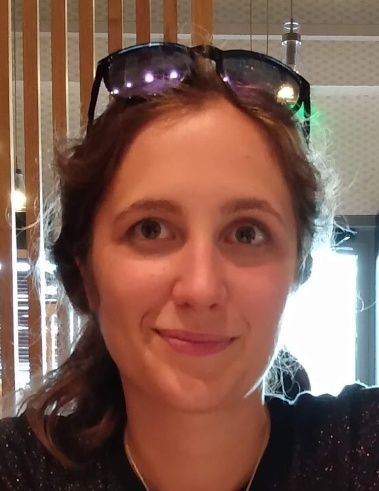
\includegraphics[height=40mm]{cecile_2}};
\end{tikzpicture}
%
%icon kubernetes
\begin{tikzpicture}[overlay, remember picture]
    \node[inner sep=0pt] (whitehead) at ([xshift=-10cm,yshift=-1cm]current page.north east)
        {
\includegraphics[height=20mm]{kubernetes}};
\end{tikzpicture}
%icon python
\begin{tikzpicture}[overlay, remember picture]
    \node[inner sep=0pt] (whitehead) at ([xshift=-7cm,yshift=-1cm]current page.north east)
        {
\includegraphics[height=20mm]{python}};
\end{tikzpicture}
%Central part
\begin{minipage}[t]{0.68\textwidth}
%
% ABOUT ME
%
\textcolor{black}{\large \bf About me \vspace{-5pt}\\}
\noindent\textcolor{blue}{\rule{13cm}{.8mm}}\\
%
\hspace*{5mm}"Lorem ipsum dolor sit amet, consectetuer adipiscing elit. Ut purus elit,
vestibulum ut, placerat ac, adipiscing vitae, felis. Curabitur dictum
gravida mauris."
%
% EXPERIENCE
%
\vspace*{1cm}\\
\textcolor{black}{\large \bf Professional experience \vspace{-5pt}\\}
\noindent\textcolor{blue}{\rule{13cm}{.8mm}}\\
%
\vspace*{-5pt}\\
\textcolor{blue}{\bf \textit{EPSILON - Group ALCEN / Toulouse}}\hfill\textcolor{gray!40}{\rule{5cm}{2mm}}\\
\begin{tabular}{P{2.5cm}p{10cm}}
\textcolor{black}{\bf 2019 - Now} & \textcolor{black}{\bf Containerized sofware developer \& integrator}
\begin{itemize}
  \item \small \textcolor{gray}{Task 1}
  \item \small \textcolor{gray}{Task 2}
\end{itemize}\\
\textcolor{black}{\bf 2017 - 2019} & \textcolor{black}{\bf DevOps sofware developer}
\begin{itemize}
  \item \small \textcolor{gray}{Task 1}
  \item \small \textcolor{gray}{Task 2}
\end{itemize}\\
\end{tabular}
\textcolor{blue}{\bf \textit{ALTRAN Technologies / Blagnac}}\hfill\textcolor{gray!40}{\rule{5cm}{2mm}}\\
\begin{tabular}{P{2.5cm}p{10cm}}
\textcolor{black}{\bf 2017(6 mo.)} & \textcolor{black}{\bf Thermal analysis optimization (Intern)}
\begin{itemize}
  \item \small \textcolor{gray}{Task 1}
  \item \small \textcolor{gray}{Task 2}
\end{itemize}\\
\end{tabular}
%
% DIPLOMA & CERTIF
%
\vspace*{1cm}\\
\textcolor{black}{\large \bf Diploma \& Certificates \vspace{-5pt}\\}
\noindent\textcolor{blue}{\rule{13cm}{.8mm}}\\
%
\vspace*{-5pt}\\
\begin{tabular}{P{2.5cm}p{10cm}}
\textcolor{black}{\bf 2020} & \textcolor{black}{ \bf Certificate - Kubernetes Certified Administrator (KCA)}  \newline \small \textcolor{gray}{Udemy} \\
\textcolor{black}{\bf 2020} & \textcolor{black}{ \bf Certificate - Kubernetes Certified Application Developer (KCAD)} \newline \small \textcolor{gray}{Udemy} \\
\textcolor{black}{\bf 2017} & \textcolor{black}{ \bf Certificate - Engineer Degree \& Master Degree} \newline \small \textcolor{gray}{IPSA} \\
\end{tabular}
%
% LANGUAGES
%
\vspace*{1cm}\\
\textcolor{black}{\large \bf Languages \vspace{-5pt}\\}
\noindent\textcolor{blue}{\rule{13cm}{.8mm}}\\
%
\vspace*{-5pt}\\
\begin{tabular}{p{2.5cm}p{10cm}}
\textcolor{black}{\bf French} & \textcolor{black}{ Native } \\
\textcolor{black}{\bf English} & \textcolor{black}{ Fluent } \\
\textcolor{black}{\bf German} & \textcolor{black}{ Basic } \\
\end{tabular}
\end{minipage}
%
\begin{minipage}[t]{0.02\textwidth}
\hspace{1mm}
\end{minipage}
%Side part
\begin{minipage}[t]{0.25\textwidth}
%
% CONTACT
%
\vspace{2cm}
\textcolor{white}{\bf \MineSign \hfill 3+ yrs of exp}\\
\textcolor{white}{\bf \Info \hfill 26 yrs-old}\\
\textcolor{white}{\bf \Telefon \hfill +33 6 37 44 17 61}\\
\textcolor{white}{\bf \Letter \hfill wiart.ccil@gmail.com}\\
\textcolor{white}{\bf \faHome \hfill 3 rue des bouquetins}\\
\textcolor{white}{\bf \hfill 31200 Toulouse}\\
%
% COMPETENCES
%
\vspace{4cm}
\begin{tabular}{|lc|}
\hline
\multicolumn{2}{|c|}{\cellcolor{white} \bf DevOps Techno} \\
\hline
\cellcolor{white} Docker & \cellcolor{white}\podrate{5}{5} \\
\cellcolor{white} Kubernetes & \cellcolor{white}\podrate{4}{5} \\
\hline
\multicolumn{2}{c}{} \\
\hline
\multicolumn{2}{|c|}{\cellcolor{white} \bf DevOps Components} \\
\hline
\cellcolor{white}Git & \cellcolor{white}\podrate{5}{5} \\
\cellcolor{white}Jenkins & \cellcolor{white}\podrate{5}{5} \\
\cellcolor{white}Artifactory & \cellcolor{white}\podrate{5}{5} \\
\cellcolor{white}Sonarqube & \cellcolor{white}\podrate{4}{5} \\
\hline
\multicolumn{2}{c}{} \\
\hline
\multicolumn{2}{|c|}{\cellcolor{white} \bf Front end} \\
\hline
\cellcolor{white}Angular & \cellcolor{white}\podrate{3}{5} \\
\cellcolor{white}HTML & \cellcolor{white}\podrate{4}{5} \\
\cellcolor{white}CSS & \cellcolor{white}\podrate{4}{5} \\
\hline
\multicolumn{2}{c}{} \\
\hline
\multicolumn{2}{|c|}{\cellcolor{white} \bf Back end} \\
\hline
\cellcolor{white}Python & \cellcolor{white}\podrate{5}{5} \\
\cellcolor{white}Node.js & \cellcolor{white}\podrate{3}{5} \\
\hline
\multicolumn{2}{c}{} \\
\hline
\multicolumn{2}{|c|}{\cellcolor{white} \bf Database} \\
\hline
\cellcolor{white}MongoDB & \cellcolor{white}\podrate{3}{5} \\
\hline
\end{tabular}
\end{minipage}
\end{document}